\section{Graphische Überlagerung von $\sin$ und $\cos$}
Es wurden ein Sinus und ein Kosinus überlagert, wie gefordert sind die Werte für
die Amplitude ($A$) und den Phasenversatz ($x_0$) abgelesen. Die exakten Werte
sind $A = \sqrt 2$ und $\frac{\pi}{4}$, wie man aus einer einfachen Rechnung
erhält, unter der Annahme, dass wir bereits wissen, dass wieder ein Sinus
herauskommt. Dann haben wir nämlich genau die beiden genannten Freiheitsgrade.
Die Amplitude ist das Maximum der Funktion, der Phasenversatz die Stelle, an der
dieses Maximum angenommen wird:
\begin{align*}
    &\frac{\mathrm d}{\mathrm dx}(\cos(x) + \sin(x)) = 0 \\
    \Leftrightarrow \quad & \sin(x) = \cos(x) \\
    \Leftrightarrow \quad & x = n\pi + \frac{\pi}{4},\ n\in\mathrm Z \\
                          & f(x) = \sqrt 2
\end{align*}

\lstinputlisting[language=Gnuplot]{4_ueberlagerung.gp}

\begin{figure}[h!]
  \begin{center}
    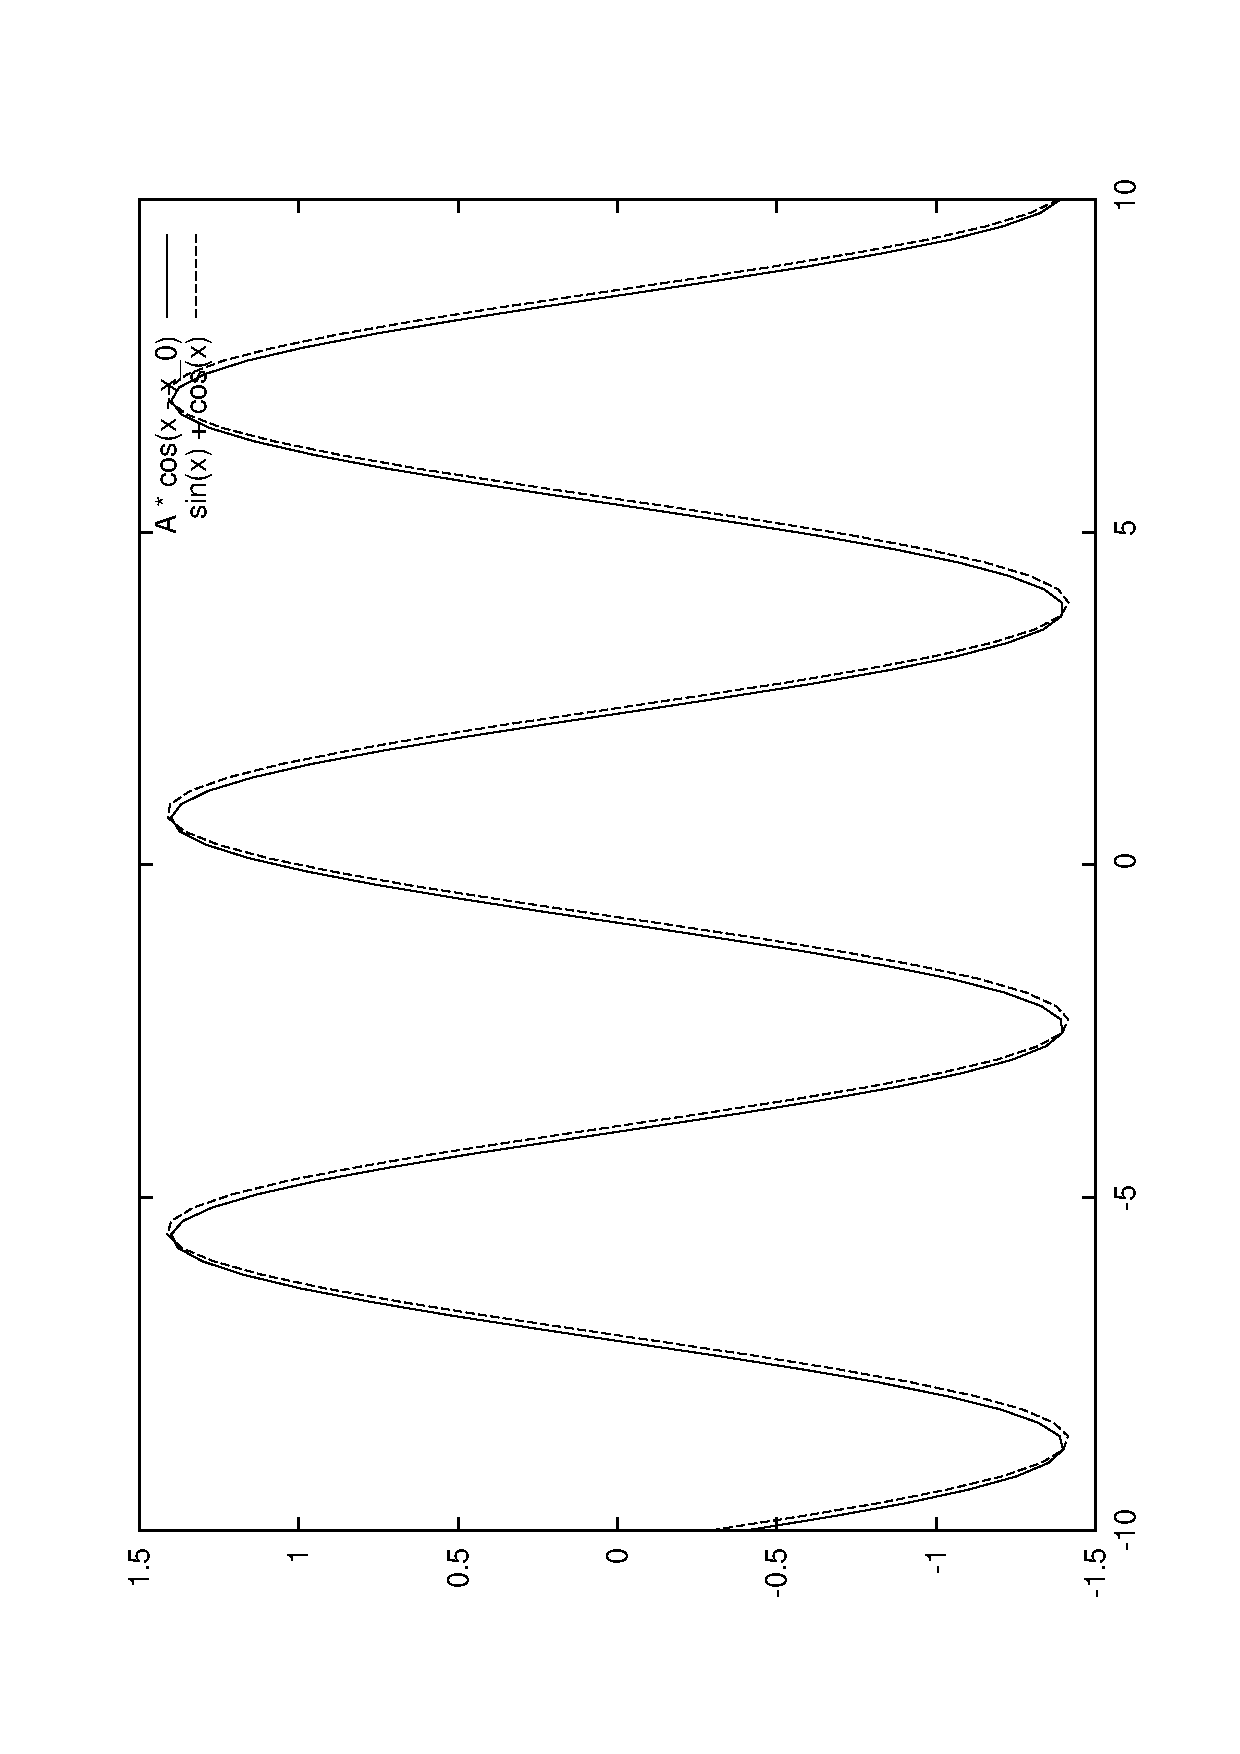
\includegraphics{grafiken/vergleich}
  \end{center}
  \caption{Vergleich des exakten Graphen mit dem "`Geratenen"'}
  \label{fig:vergleich}
\end{figure}

